\documentclass{automatextcc}
\usepackage{ulem}
\usepackage{dsfont}
\usepackage{placeins}

% Caminho da Pasta das Figuras
\graphicspath{{figuras/}}

%\makeindex  Opcional (Índice Remissivo)

\newcommand{\pumi}[1]{\textcolor{red}{#1}}
\newcommand{\R}{\mathds{R}}
\newcommand{\N}{\mathds{N}}
\newcommand{\bs}[1]{\boldsymbol{#1}}
\begin{document}


\title{Composição Automática de Músicas utilizando Redes Neurais Recorrentes}
\author{Nicolas Mathias Hahn}

% orientador(a) do trabalho {nome}{Orientador(a)}
\advisor{Prof. Dr. Guilherme Pumi}{Orientador}
% universidade onde obteve o título e atual
\advisorinfo{Doutor pela Universidade Federal do Rio Grande do Sul, Porto Alegre, RS}{UFRGS}

% banca examinadora:
\examinera{Prof. Dr. xxx}
\examinerainfo{Doutor pela XX -- Cidade, Estado}{Universidade}

% departamento:
\dept{\DEST}

% data de entrega:
\date{Outubro de 2022}


% Capa
\maketitulo

% Folha de rosto
\makefolhaderosto

% Folha de aprovação
\makefolhadeaprovacaoA % Um membro na banca
%\makefolhadeaprovacaoB % Dois membros na banca


% Epígrafe (OPCIONAL)
\newpage
\vspace*{\fill}
\begin{flushright} % mexer aqui
	\textit{``Since I have always preferred making plans to executing them, I have gravitated towards situations and systems that, once set into operation, could create music with little or no intervention on my part. That is to say, I tend towards the roles of planner and programmer, and then become an audience to the results.''} \newline
	\textit{Brian Eno \citep{alpern1995}}.
\end{flushright}

% Agradecimentos
\newpage
\chapter*{Agradecimentos}
Agradeço a xxx. Opcional % mexer aqui

% palavras chave
    % português
\keyword{Redes Neurais}
\keyword{Música}
    % inglês
\keyworde{Neural Networks}
\keyworde{Music}

% resumo 
    % português
\begin{abstract}
Este trabalho ....
\end{abstract}
    % inglês
\begin{englishabstract}
In this work ....
\end{englishabstract}

% sumário (Obrigatório)
\tableofcontents

% lista de ilustrações (Obrigatório)
\listoffigures

% lista de tabelas (Obrigatório)
\listoftables

% se um pato perde a pata, ele fica manco ou viúvo???

% Regras do PUMI:
%  * vamos ver a introdução por último
%  * deixar em bullets os itens que pretende falar
%  * focar na fundamentação teórica (redes neurais, RNN e LSTM)


%%%%%%%%%%%%%%%%%%%%%%%%%%%%%%%%%%%
%%%%  Introdução
%%%%%%%%%%%%%%%%%%%%%%%%%%%%%%%%%%%
\chapter{Introdução}

\begin{itemize}
    \item composição algorítmica (composição automática) - caminhar histórico?
    \item formas de composição algorítmica: rule-based, stochastic e AI
\end{itemize}

% certamente olhar este artigo e suas bibliografias:
% https://ccrma.stanford.edu/~blackrse/algorithm.html

% talvez olhar este artigo:
% https://musica.ufmg.br/nasnuvens/wp-content/uploads/2020/11/2016-38-A-interatividade-nas-trilhas-sonoras-de-jogos-digitais-e-um-comparativo-com-a-música-de-cinema.pdf



% referencial teórico
\chapter{Referencial Teórico}

    % NN
\section{Redes Neurais Artificiais}
    % aggarwal 2018
%Redes Neurais Artificiais são técnicas populares de aprendizagem de máquina que simulam o mecanismo de aprendizagem presente em organismos vivos.
    % haykin 2002
%O trabalho em redes neurais artificiais, usualmente denominadas "redes neurais", tem sido motivado desde o começo pelo reconhecimento de que o cérebro humano processa informações de uma forma diferente do computador digital convencional. O cérebro é um computador (sistema de processamento de informação) altamente complexo, não linear e paralelo. Ele tem a capacidade de organizar seus constituintes estruturais, conhecidos por neurônios, de forma a realizar certos processamentos (ex. reconhecimento de padrões, percepção e controle motor) muito mais rapidamente que o mais rápido computador digital hoje existente.
    % elements of statistical learning 2008
%O termo "rede neural" tem evoluído para abranger uma grande classe de modelos e métodos de aprendizagem. [...] Elas são apenas modelos estatísticos não lineares.
    % goodfellow 2016
%Alguns dos algoritmos iniciais que reconhecemos hoje tinham o intuito de ser um modelo computacional da aprendizagem biológica, i.e., modelos de como a aprendizagem poderia ocorrer no cérebro. A correspondente perspectiva de deep learning (redes neurais artificiais) é que são engineered systems inspirados pelo cérebro (seja humano seja de outro animal)
    % hair et al 2005
%Redes neurais são uma abordagem totalmente diferente para a análise de dados em relação a qualquer outra técnica multivariada. Em vez de conceitualizar o problema como de caráter matemático, redes neurais usam o cérebro humano e sua estrutura para desenvolver uma estratégia de processamento. Apesar de jamais sermos capazes de construir redes neurais tão complexas quanto o cérebro humano, podemos usar seus princípios básicos de unidades de processamento paralelo múltiplo engajadas no reconhecimento de padrões. 

% paragrafo
Redes Neurais Artificiais (RNA) são técnicas de aprendizagem de máquina inspiradas no mecanismo de aprendizagem presente em organismos vivos \citep{aggarwal2018} sendo que, nos seus primórdios, os algoritmos tinham o intuito de ser um modelo computacional capaz de imitar a aprendizagem ocorrida no cérebro \cite{goodfellow2016}.  Por outro lado, RNAs podem ser vistas como modelos estatísticos não lineares \citep{hastie2009}.

\subsection{Deep Learning}

\begin{itemize}
    \item renascimento de redes neurais 
    \item deep learning são redes neurais profundas (com muuuitas camadas)
\end{itemize}


\subsection{Redes Neurais e a Estatística}
Muitos modelos de RNAs são similares ou idênticos a populares técnicas estatísticas como modelos lineares generalizados, regressão linear (simples e múltipla), regressão polinomial, regressão não paramétrica e análise discriminante (como a regressão logística) entre outros, especialmente quando a ênfase é na predição de um fenômeno complexo em vez de sua explicação \citep{sarle1994, cheng1994}.

\pumi{Esta sentença está ruim} No contexto de RNAs, dois aspectos de tratamento podem ser definidos a um problema prático: (i) especificar a arquitetura da rede; (ii) treinar a rede para performar bem com o conjunto de treinamento (referencial). Para o estatístico, tais passos são equivalentes a: (i) especificar um modelo de regressão; (ii) estimar os parâmetros do modelo dado um conjunto de dados. Por conseguinte, uma RNA pode ser pensada como uma generalização não linear de um modelo linear, seja para regressão, seja para classificação \citep{cheng1994, hastie2009}. 


\subsubsection{Jargões} 
Apesar de muitos modelos de RNAs serem similares ou idênticos a modelos estatísticos, os termos na literatura de RNAs são diferentes da estatística. \pumi{No que segue apresentamos uma lista não exaustiva de termos comumente utilizados na literatura de RNAs e suas equivalências em estatística:}

\begin{itemize}
    \item variables are called features
    \item independent variables are called input
    \item predicted values are called output
    \item dependent variables are called targets or training values
    \item residuals are called errors
    \item estimation is called training, learning, adaptation, or selforganization
    \item an estimation criterion is called an error function, cost function, or Lyapunov function
    \item observations are called patterns or training pairs
    \item parameter estimates are called (synaptic) weights
    \item interactions are called higher-order neurons
    \item transformations are called functional links
    \item regression and discriminant analysis are called supervised learning or heteroassociation
    \item data reduction is called unsupervised learning, encoding, or autoassociation
    \item cluster analysis is called competitive learning or adaptative vector quantization
    \item interpolation and extrapolation are called generalization
\end{itemize}
Os termos estatísticos amostra e população não demonstram conter equivalentes na literatura de RNAs. No entanto, os dados são comumentes divididos em conjunto de treino e de teste para validação cruzada \citep{cheng1994}.


\subsection{Neurônio}
Um neurônio (ou nó computacional) é uma unidade de processamento de informação fundamental para a operação de uma rede neural \citep{haykin2001}. Podemos identificar três elementos básicos do modelo neuronal:
\begin{enumerate}
    \item Um conjunto de sinapses, cada uma caracterizada por um peso ou força própria. O peso sináptico de um neurônio artificial pode estar em um intervalo que inclui valores positivos e negativos.
    \item Um \textit{somador} ou \textit{acumulador} para somar os sinais de entrada, ponderados pelas respectivas sinapses de cada neurônio, constituindo uma \textit{combinação linear}.
    \item Uma \textit{função de ativação} para restringir a amplitude de saída de um neurônio (fixando em um valor finito).
\end{enumerate}
Também é incluído um \textit{bias} (viés) no modelo, externo ao neurônio, com o intuito de aumentar ou diminuir a entrada da função de ativação, dependendo do seu sinal.

Matematicamente, podemos descrever um neurônio $k \in \N$, por meio de um par de equações:
\begin{align*}
    y_k &= \varphi(u_k + b_k) = \varphi(v_k);\\[.2cm]
    u_k &= \displaystyle{\sum_{i=1}^{m} }w_{k,i}x_i;
\end{align*}
em que $x_i \in \R$, $i \in \{1,\dots,m\}$, $m \in \N$, são os valores observados; $w_{k,i} \in \R$, são os pesos associados ao neurônio $k$; $u_k$ é a saída da combinação linear entre os sinais de entrada e os pesos; $b_k$ é o \textit{bias}; $\varphi(\cdot)$ é uma função de ativação; e $y_k$ é o sinal de saída.

\begin{figure}
    \centering
    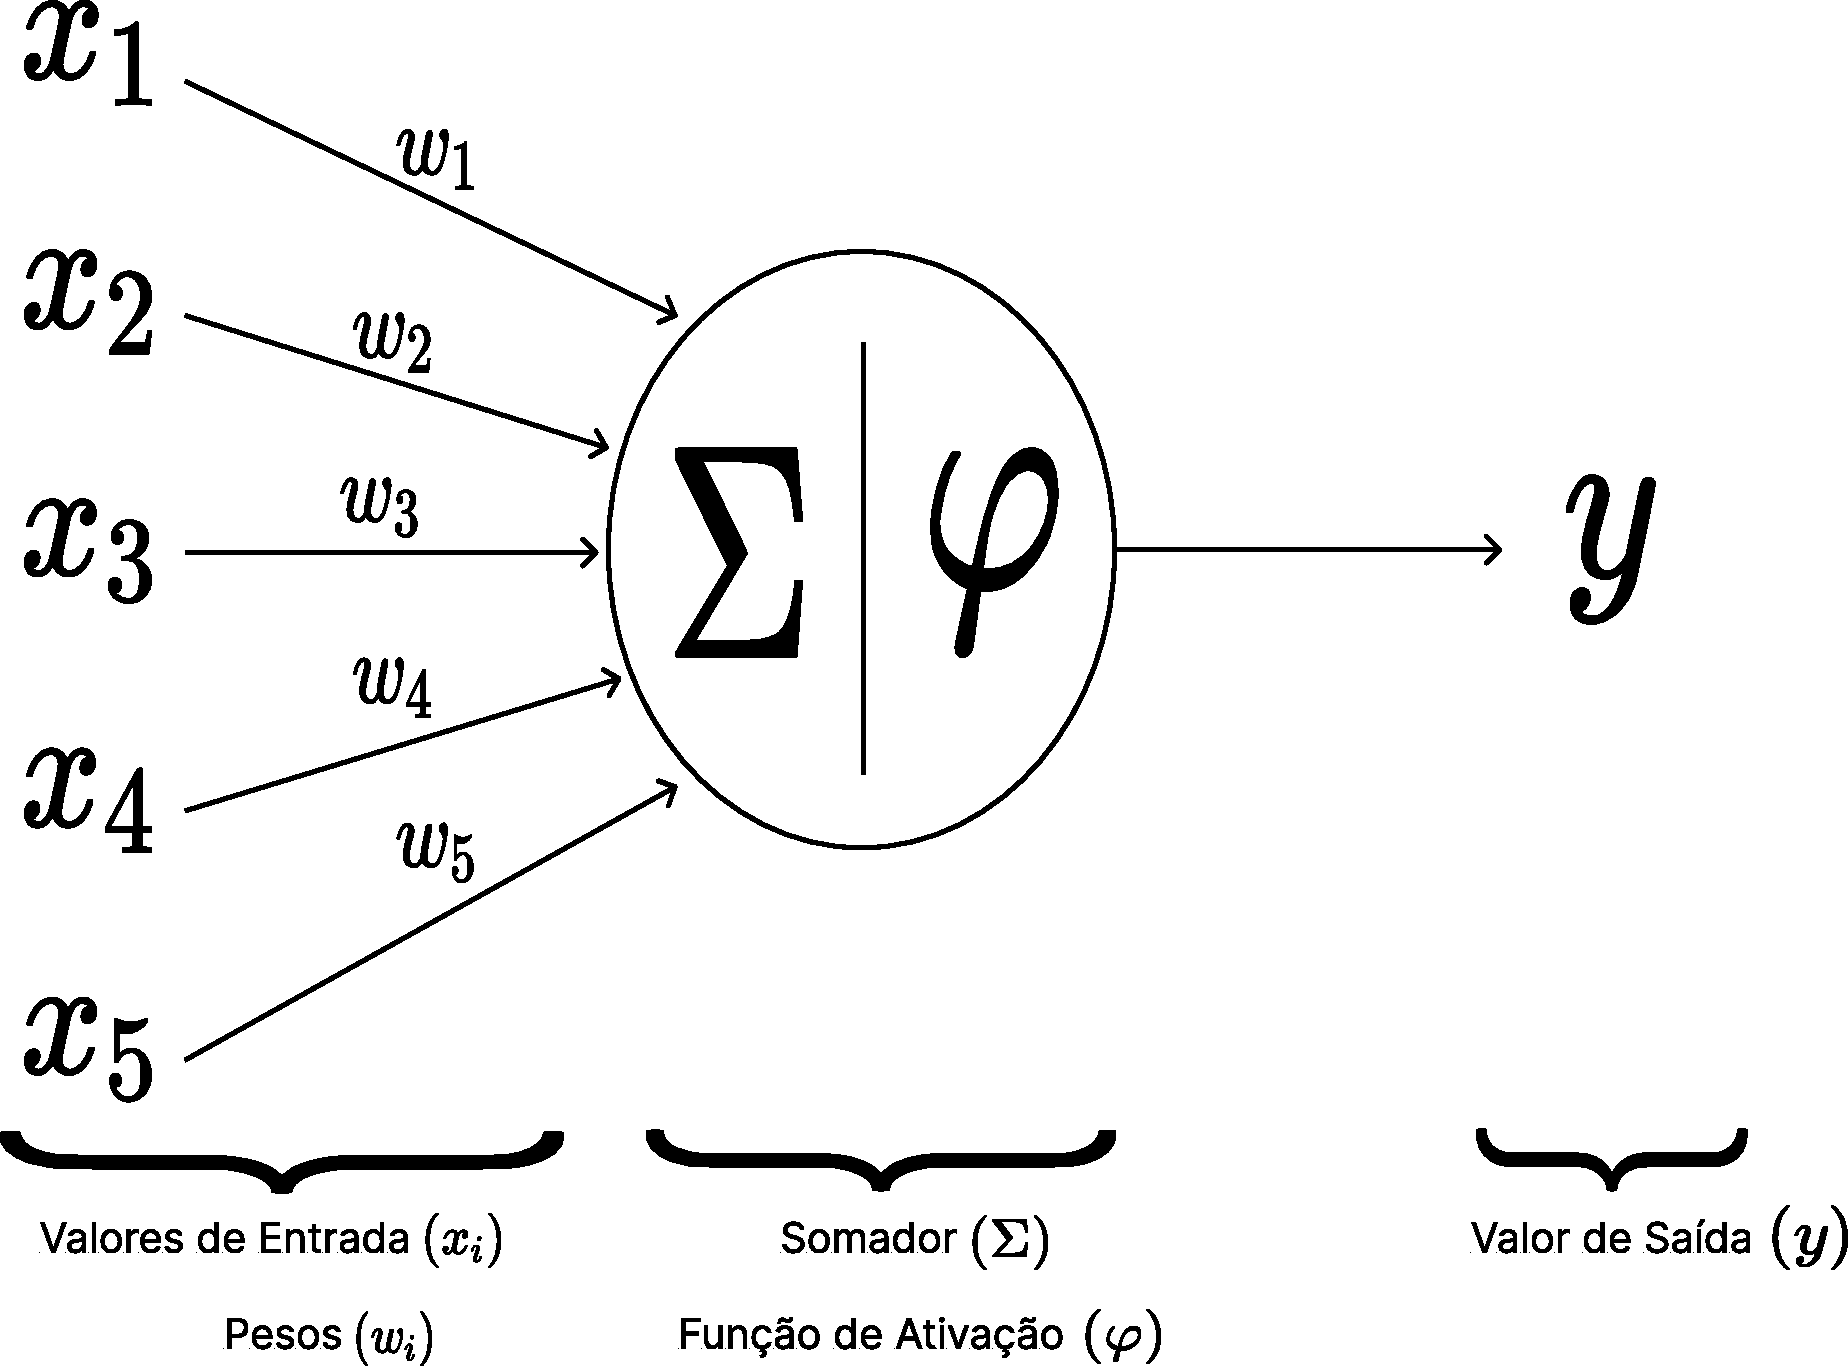
\includegraphics[width=.7\textwidth]{figuras/neuron_model.pdf}
	\caption{Modelo Neuronal (adaptado de \citet{haykin2001,hair2005})}
\end{figure}

\subsection{Função de Ativação}
O objetivo da função de ativação (ou de transferência) é determinar se a informação que o neurônio está recebendo será passada adiante ou será ignorada \citep{dsa2022}. \citet{hagan2014} comenta que uma função de ativação particular é selecionada para satisfazer uma determinada especificação do problema que o neurônio almeja resolver. Assim, temos que a função de ativação pode ser linear ou não-linear. Abaixo, seguem algumas funções de ativação:

\begin{itemize}
    \item \textbf{linear:} $f: \R \rightarrow \R$ dada por $f(x) = \alpha x,$  $\alpha \in \R\backslash\{0\}$. \\
    Observe que no caso da função linear, o neurônio está sempre ativado, sendo seu valor alterado pela constante $\alpha$. Em particular, quando $\alpha=1$, temos a função identidade e, como comenta \citet{sarle1994}, um modelo de regressão linear.
    \item \textbf{sigmóide ou \textit{logit}}: $f: \R \rightarrow (0,1)$ dada por $f(x) = \frac{1}{1 + e^{-x}}$. \\
    Quando \sout{a rede tem} essa função de ativação \pumi{é associada a uma rede}, o neurônio \pumi{é equivalente a uma} \sout{um modelo linear generalizado conhecido como} regressão logística. Dessa forma, notamos que a função de ativação tem um papel semelhante à função de ligação \pumi{no contexto de modelos lineares gerais}: relacionar o preditor linear \pumi{ao respectivo valor esperado} \sout{$v$ a um valor esperado $\mu$ de um dado $y$} \citep{sarle1994,frei2020,mccullagh1989}. % ficou meio jogado?
    \item \textbf{tangente hiperbólica (\textit{tanh}):}  $f:\R \rightarrow (-1,1)$ dada por $f(x) = \frac{e^{x}-e^{-x}}{e^{x}+e^{-x}}$. \\
    Em contextos que uma função sigmoidal é necessária (como a predição de uma variável binária), a \textit{tanh} tipicamente performa melhor. Vale comentar que funções de ativação sigmoidal são mais comuns em estruturas diferentes que a de redes alimentadas adiante, como as redes recorrentes \citep{goodfellow2016}.  
    \item \textbf{ReLU (\textit{Rectified Linear Unit}):} $f: \R \rightarrow [0,\infty)$ dada por $f(x) = \max\{0,x\}$. \\
    De acordo com \citet{goodfellow2016}, é a recomendação padrão para redes neurais modernas. O autor justifica que, por ser uma função quase linear, são preservadas muitas propriedades que fazem os modelos lineares bons generalizadores. % pq? % quais? 
\end{itemize}
% pq domínio é igual para todos?
Listas de funções de ativação comumente utilizadas podem ser encontradas em \citet{hagan2014}, \citet{aggarwal2018} e \citet{dsa2022}.


\subsection{Arquiteturas de RNAs}
%Comumente, um neurônio, mesmo com muitas entradas, pode não ser suficiente. Talvez sejam necessários cinco ou dez, operando paralelamente, no que chamamos de ``camada''. Alguns autores referem-se às entradas como outra camada, mas não faremos isso aqui \citep{hagan2014}. 
%Em geral, podemos identificar três classes de arquiteturas de rede fundamentalmente diferentes \citep{haykin2001}.

% A rede neural é um arranjo sequencial de três tipos básicos de nós ou camadas: nós de entrada (ou fonte, como comenta \citet{haykin2001}), nós de saída e nós intermediários (ocultos). Os nós de entrada recebem os valores iniciais de dados de cada caso e os transmitem para a rede neural. Um nó de entrada representa uma única variável ou padrão. Variáveis métricas demandam apenas um nó para cada variável. Variáveis não-métricas devem ser codificadas, significando que cada categoria é representada por uma variável binária (exatamente o processo de criação de uma variável dicotômica ou \textit{dummy}, mas sem a eliminação de uma categoria de referência). 
%Um nó de saída recebe entradas e calcula um valor de saída, mas em vez de ir para outro nó, esse é o valor final. Se esse for um modelo preditivo, então esse valor é o resultado da previsão. Se o modelo é utilizado para classificação, então esse é o valor empregado no processo de classificação (que será utilizado para determinar qual categoria foi classificada). 
%\citep{hair2005}.

Um único neurônio (nó computacional), mesmo com muitas entradas, usualmente não é suficiente \pumi{para o quê?}, sendo necessários cinco ou dez operando paralelamente em uma estrutura que chamamos de ``camada''. Temos que uma rede neural é constituída por três tipos básicos de camadas:

\begin{enumerate}
    \item \textbf{Entrada:} constituída por nós de fonte, em que cada nó representa uma variável independente $x_i$. Vale comentar que variáveis numéricas requerem apenas um nó, porém variáveis categóricas requerem um nó para cada categoria, semelhantemente ao processo de criação de variáveis dicotômicas ou \textit{dummies}, mas sem a eliminação de uma categoria de referência.
    \item \textbf{Saída:} composta por neurônios, com a diferença que seu valor de saída é definitivo. No caso de um modelo preditivo, o valor será o resultado da previsão. Se o modelo é utilizado para classificação, então o valor resultante será empregado no processo de classificação (que será utilizado para determinar qual categoria foi classificada).
    \item \textbf{Intermediária ou oculta:} assim como a camada de saída, é composta por neurônios. Suas valores de entrada podem ser originados da camada de entrada ou da camada oculta anterior, bem como seus valores de saída podem alimentar a próxima camada oculta ou a camada de saída.
\end{enumerate}
Posto isso, organizamos as redes em três arquiteturas fundamentalmente diferentes \citep{haykin2001,hair2005,hagan2014}: redes alimentadas adiante com camada única, com múltiplas camadas e redes recorrentes.


\subsubsection{Redes Alimentadas Adiante}

%Em uma rede neural em camadas, os neurônios estão organizados na forma de camadas. Na forma mais simples de uma rede em camadas, temos a camada de entrada de nós de fonte que se projeta sobre uma camada de saída de neurônios (nós computacionais), mas não vice-versa. Em outras palavras, esta rede é estritamente do tipo alimentada adiante ou acíclica. [...]. Esta rede é chamada de camada única sendo que a designação ``camada única'' se refere à camada de saída de nós computacionais (neurônios). Não contamos a camada de entrada de nós de fonte, porque lá não é realizada nenhuma computação \citep{haykin_2001}.

%A nomenclatura alimentada adiante é devido ao fluxo de informação ser avaliado desde a camada de entrada $\bs{x}$, através de computações intermediárias realizadas na(s) camada(s) oculta(s) $\bs{h}$ até a camada de saída $\bs{y}$. Não há nenhuma conexão de realimentação em que as saída do modelos são inseridas como entradas no próprio modelo. Quando há tais alimentações, temos redes neurais recorrentes     \citep{goodfellow2016}

% The most widely used ``vanilla'' neural net, sometimes called the single hidden layer back-propagation network or single layer perceptron \citep{hastie2009}. 


%A segunda classe de uma rede neural alimentada se distingue pela presença de uma ou mais camadas ocultas, cujos nós computacionais são chamados correspondentemente de neurônios ocultos ou unidades ocultas. A função dos neurônios ocultos é intervir entre a camada externa e a saída da rede de uma maneira útil. Adicionando-se uma ou mais camadas ocultas, tornamos a rede capaz de extrair estatísticas de ordem elevada. Em um sentido bastante livre, a rede adquire uma perspectiva global apesar de sua conectividade local, devido ao conjunto extra de conexões sinápticas e da dimensão extra de interações neurais (Churland e Sejnowski, 1992). A habilidade de os neurônios ocultos extraírem estatísticas de ordem elevada é particularmente valiosa quando o tamanho da camada de entrada é grande \citep{haykin2001}.

%Os nós de fonte da camada de entrada da rede fornecem os respectivos elementos do padrão de ativação (vetor de entrada), que constituem os sinais de entrada aplicados aos neurônios (nós computacionais) na segunda camada (i.e., primeira camada oculta). Os sinais de saída da segunda camada são utilizados como entradas para a terceira camada, e assim por diante para o resto da rede. Tipicamente, os neurônios em cada camada da rede têm como suas entradas apenas os sinais de saída da camada precedente. O conjunto de sinais de saída (final) da rede constitui a resposta global da rede para o padrão de ativação fornecido pelos nós de fonte da camada de entrada (primeiro). [...]. Como um outro exemplo, uma rede alimentada adiante com $m$ nós de fonte, $h_1$ neurônios na primeira camada oculta, $h_2$ neurônios na segunda camada oculta e $q$ neurônios na camada de saída é referida como uma rede $m-h_1-h_2-q$ \citep{haykin2001}.

%A rede neural é dita totalmente conectada, no sentido de que cada um dos nós de uma camada da rede está conectado a todos os nós da camada adjacente seguinte. Entretanto, se alguns dos elos de ligação (conexões sinápticas) estiverem faltando na rede, dizemos que a rede é parcialmente conectada  \citep{haykin2001}.

A nomenclatura desse tipo de arquitetura é devida ao fluxo de informação partir da camada de entrada até a camada de saída, de forma unidirecional \citep{goodfellow2016}. \citet{hastie2009} e \citet{fan2021} comentam que é o tipo padrão de rede neural. A principal diferença entre uma rede de camada única e uma com múltiplas camadas é a existência (ou não) das camadas ocultas, sendo que a designação ``camada única'' se refere a uma camada de neurônios ou nós computacionais. Além disso, há a distinção entre a rede ser totalmente ou parcialmente conectada, no sentido de que os nós de uma camada são conectados a todos os nós da camada adjacente \citep{haykin2001}. 
% vanilla == padrão (não encontrei sinônimo bom, talvez trocar para "básica")

\begin{itemize}
    \item imagens com rede camada única e camada múltipla
    \item imagens com rede totalmente e parcialmente conectada
\end{itemize}

\subsubsection{Redes Neurais Recorrentes}
%Uma rede neural recorrente se distingue de uma rede neural alimentada adiante por ter pelo menos um laço de realimentação. Uma rede recorrente pode consistir, por exemplo, de uma única camada de neurônios com cada neurônio alimentando seu sinal de volta para as entradas de todos os outros neurônios. [...]; auto-realimentação se refere a uma situação onde a saída de um neurônio é realimentada para a sua própria entrada. [...]. \citep{haykin2001}

%A presença de laços de realimentação, [...], tem um impacto profundo na capacidade de aprendizagem da rede e no seu desempenho. Além disso, os laços de realimentação envolvem o uso de ramos particulares compostos de elementos de atraso unitário (representado por $z^{-1}$), o que resulta em um comportamento dinâmico não-linear, admitindo-se que a rede contenha unidades não-lineares. \citep{haykin2001}

%One important characteristic is weight sharing that is some model parameters are identical across time. This is related to the notion of stationarity.
%Recurrent neural nets (RNN) are designed to process time series data or other sequence data. Here, we introduce vanilla RNNs and improved variants such as long short-term memory (LSTM).
%Recurrent neural nets (RNN) are models designed to process time series data and other sequence data.
%Note that in different applications, we may have different input/output settings. Examples include one-to-many, many-to-one and many-to-many.
%One notable drawback of vanilla RNNs is that they have difficulty in capturing long-range dependencies in sequence data when the length of the sequence is large. This is sometimes due to the phenomenon of exploding/vanishing gradients.
%gated recurrent units (GRU) and long short-term memory (LSTM).
%\citep{fan2021}

%Parameter sharing makes it possible to extend and apply the model to examples of different forms (different lengths, here) and generalize across them. If we had separate parameters for each value of the time index, we could not generalize to sequence lenghts and across different positions in time. Such sharing is particularly important when a specific piece of information can occur at multiple positions within the sequence.
%For the simplicity of exposition, we refer to RNNs as operation on a sequence that contains vectors $\bs{x}^{(t)}$ with the time step index $t$ ranging from 1 to $\tau$. In practice, RNN usually operate on minibatches of such sequences, with a different sequence length $\tau$ for each member of the minibatch. We have omitted the minibatch indices to simplify notation. Moreover, the time step index need not literally refer to the passage of time in the real world. Sometimes it refers only to the position in the sequence. 
%citep{goodfellow2016}

%Recurrent neural networks (RNNs) are designed for sequential data like text sentences, time-series and other discrete sequences like biological sequences. In these cases, the input is of the form $\bs{x}^{(1)},\dots,\bs{x}^{(T)}$, where $\bs{x}^{(t)}$ is a $d$-dimensional point received at the time-stamp $t$. For example, the vector $\bs{x}^{(t)}$ might contain the $d$-values of at the $t$th tick of a multivariate time-series (with $d$ different time-series). In a text-setting, the vector $\bs{x}^{(t)}$ will contain the one-hot encoded word at the $t$th time-stamp. In one-hot encoding, we have a vector of length equal to the lexicon size, and the component for the relevant word has a value of 1. All other components are 0.
%An important point about sequences is that successive words are depedent on one another. [...]. The traditional type of feed-forward network in which all inputs feed into the first layer dows not achieve this goal. Therefore, the RNNs allow the input $\bs{x}^{(t)}$ to interact directly with the hidden state created from the inputs at previous time-stamps. [...]. The key point is that there is an input $\bs{x}^{(t)}$ at each time-stamp, and a hidden state$\bs{h}^{(t)}$ that changes at each time-stamp as new data points arrive. Each time-stamp also has an output value $\bs{y}^{(t)}$. For example, in a time-series setting, the output $\bs{y}^{(t)}$ might be the forecasted prediction of $\bs{x}^{(t+1)}$. When used in the text-setting of predicting the next word, this approach is called language modelling. In some applications, we do not output $\bs{y}^{(t)}$ at each time-stamp, but only at the end of the sequence. For example, if one is trying to classify the sentiment of a sentence as ``positive'' or ``negative'', the output will occur only at the final time-stamp.
%The hidden state at time $t$ is given by a function of the input vector at time $t$ and the hidden vector at time $t-1$: $\bs{h}^{(t)} = f(\bs{h}^{(t-1)},\bs{x}^{(t)})$.
%A key point here is the presence of the self-loop, which will cause the hidden state of the neural network to change after the input of each $\bs{x}^{(t)}$. In practice, one only works with sequences of finite length, and it makes sense to unfurl the loop in a ``time-layered'' network that looks more like a feed-forward network. Note that in this case, we have a different node for the hidden state at each time-stamp and the self-loop has been unfurled into a feed-forward network. This representation is mathematically equivalent, but is much easier to comprehend because of its similarity to a traditional network.
%\citep{aggarwal2018}

Redes neurais recorrentes (RNNs) são um tipo de redes neurais criadas para processar séries temporais e outros tipos de dados sequenciais \citep{fan2021}. O que difere uma rede recorrente de uma rede alimentada adiante é seu laço de realimentação. Por exemplo, uma rede recorrente pode consistir de uma única camada de neurônios com cada neurônio alimentando seu sinal de volta para as entradas de todos os outros neurônios \citep{haykin2001}. Vamos introduzir as RNNs base, bem como variantes melhoradas como a \textit{long short-term memory} (LSTM).

%\subsubsubsection{}

%puramente copiado e sem polimento de \citep{fan2021}
\begin{itemize}
    \item \textbf{RNNs base:} suponha que $\bs{x}^{(1)},\dots,\bs{x}^{(T)}$ são entradas de uma série temporal. Uma RNN base modelo o ``estado oculto'' no tempo $t$ por meio de um vetor $\bs{h}^{(t)}$, que é utilizado na fórmula recursiva 
    \begin{equation}
        \label{recursive_formula}
        \bs{h}^{(t)} = f_{\bs{\theta}} (\bs{h}^{(t-1)},\bs{x}^{(t)}).
    \end{equation}
    Aqui, $f_{\bs{\theta}}$ é geralmente uma função não linear parametrizada por $\bs{\theta}$. Temos que uma RNN base com apenas uma camada oculta tem a seguinte forma
    \begin{equation}
        \bs{h}_{t} = \varphi \bigl( \bs{W}_{hh} \bs{h^{(t-1)}} + \bs{W}_{xh} \bs{x^{(t)}} + \bs{b_h} \bigl)
    \end{equation}
    \begin{equation}
        \bs{z}_t = \varphi \bigl( \bs{W_{hy}} + \bs{b_z} \bigl),
    \end{equation}
    
    em que $\bs{W}_{hh}$, $\bs{W}_{xh}$, $\bs{W}_{hy}$ são  matrizes de pesos, $\bs{b}_{h}$, $\bs{b}_{z}$ são vetores de \textit{bias}, e $z_t$ é a saída no tempo $t$. Como em muitos modelos clássicos de séries temporais, esses parâmetros são compartilhados ao longo do tempo. Note que, dependendo da aplicação, podemos ter diferentes configurações de entrada e saída: \textit{one-to-many} (única entrada e múltiplas saídas), \textit{many-to-one} (múltiplas entradas e única saída), \textit{many-to-many}. 
    
    Um déficit da RNN base é sua dificuldade em capturar dependência longa nos dados em sequências compridas. Sendo assim, foram desenvolvidas variantes para contornar o problema, como a LSTM (\textit{long short-term memory}) e a GRU (\textit{gated recurrent units}).
    
    \item \textbf{GRU:} introduz \textit{gates} na fórmula recursiva \eqref{recursive_formula} de mesmo comprimento que $h^{(t)}$. Esses \textit{gates}, que pegam valores em $[0,1]$ multiplicados por $\bs{h^{(t-1)}}$, elemento-a-elemento, determinando por quanto tempo são mantidos os antigos \pumi{estados? esta explicação ficou confusa} \textit{hidden states}.
    \item \textbf{LSTM:} similarmente utiliza \textit{gates} na fórmula recursiva. Além de $\bs{h_t}$, uma LSTM mantém um \textit{cell state}, que pega valores em $\R$ \textit{elementwise} e são análogas a contadores.
    
\end{itemize}



%\begin{itemize}
%    \item \textbf{LSTM:}
%\end{itemize}



\section{Composição Algorítmica}

Composição algorítmica, ou composição automática, refere-se ao processo de criação de músicas por meio de algum processo formal com pouca ou nenhuma intervenção humana. O termo ``algoritmo'' é definido como um conjunto predeterminado de instruções com o objetivo de resolver um problema em específico com um número limitado de passos. O ``problema'' encarado por compositores é a composição musical, e as ``instruções'' predeterminadas sugerem que, uma vez que o processo é iniciado, a intervenção humana é substituída. Portanto, ``composição automática'' também descreve adequadamente esse tipo de composição musical, sendo que ``automático'' refere-se a ``qualquer coisa que pode se mover ou agir por conta própria'' \citep{alpern1995, maurer}.

De acordo com \citet{maurer}, podemos encontrar três metodologias diferentes que existem em composição algorítmica: 

\begin{itemize}
    \item estocástica: abordagem mais simples. Envolve aleatoriedade e pode ser tão simples quanto gerar uma série de notas musicais ao acaso, bem como sortear uma ordem de fragmentos de músicas para ser performada pelo músico.
    \item \textit{rule-based}: em vez de delegar decisões ao acaso como no método estocástico, um sistema \textit{rule-based} define uma ``constituição'' ou ``gramática'' (sistema formal de princípios ou regras que as possíveis frases de uma linguagem são geradas) em que o sistema deve seguir uma vez iniciado o processo de composição. 
    \item inteligência artificial (IA): similar ao ``rule-based'' no sentido de ser baseado em uma gramática pré-definida. No entanto, sistemas de IA têm a capacidade de definirem sua própria gramática. \sout{ ou, em essência, a capacidade de ``aprender''.}
\end{itemize}
Detalhamentos referentes às metodologias estão disponíveis em \citet{alpern1995}, \citet{maurer}, \citet{nierhaus2009}, \citet{fernandez2013} e \citet{hernandez2021}.  


\section{Notação ABC}
Notação ABC é um sistema popular de notação musical baseada em texto para transcrever, publicar e compartilhar músicas folclóricas, particularmente de forma \textit{online}. Criada e formalizada por \citet{walshaw1993}, o autor mantém um website, \url{abcnotation.com}, com recursos como tutoriais, programas e coleções de músicas no formato \citep{walshaw2014}.

A notação ABC é composta por duas partes: o cabeçalho, que fornece os metadados da música como o título e características da música, e o corpo, que detalha as notas musicais. Existem \textit{tags} no cabeçalho como ``T'' (título) e ``X'' (número da música) que não afetam a síntese musical de nenhuma forma. Vale notar que a notação ABC define um mapeamento entre seus caracteres e símbolos específicos de uma partitura musical, o que permite a conversão de um formato para outro \citep{agarwala2017}. 

\begin{itemize}
    \item imagem de notação ABC e partitura
\end{itemize}


\section{Web Scraping}

%Web scraping is an automated tool for finding and extracting data from on-line sources. It utilizes computer programming software and customized software code to mine data or other information from on-line sources in order to remove a copy of the data and store it in an external database for analysis.
%Web scraping is also referred to as automated data collection, web extracting, web crawling, or web content mining.
%Web scraping involves the development and use of two customized software programs – a crawler and a scraper. The crawler systematically downloads data from the Internet; then the scraper systematically pulls the relevant information (unstructured, semi-structured, or structured) from the downloadeddata, codes it, and relocates it ina database or file based on a pre-determined structure and format defined by the user. This new external database or file – populated with data originally presented on-line – is subsequently analyzed in ways the original on-line presentation of data did not support. Common software programming languages like R and Python are typically used to write the software code for both the crawler and the scraper.
%\citep{farley2017}

%Most websites define a \textit{robots.txt} file to let crawlers know of any restrictions about crawling their website. These restrictions are just a suggestion but good web citizens will follow them. The \textit{robots.txt} file is a valuable resource to check before crawling to minimize the chance of being blocked, and also to discover hints about a website's structure. More information about the \textit{robots.txt} protocol is available at \url{http://www.robotstxt.org}.
%\citep{lawson2015}

%Web crawlers are designed to retrieve web content and insert them to local repository. Crawlers are primarily used to produce a replica of all the visited pages that are later processed by a search engine that will index downloaded pages that facilitate in fast searches. 
%Web crawler is an internet service that assists users in their web navigation by automating the task of link traversal, making a searchable index of the web, and fulfilling searchers’ queries from the index. That is, a web crawler automatically discovers and collects different resources in an orderly fashion from the internet according to the user requirements
%\citep{patil2016}

%Web scraping or web crawling refers to the procedure of automatic extraction of data from websites using software.
%Web scraping or web crawling on the other hand is far faster and more effective, and can be used to gather and compile data from across thousands, or over millions, of pages for processing and drawing information from.
%For the vast majority of computer users, interaction with the internet comes in the form of accessing websites through a browser, where information and multimedia objects are displayed in a human-friendly fashion for easy understanding. 
%\citep{khder2021}
\pumi{web scraping = procedimento, web crawler = ferramenta}

\textit{Web scraping} (ou \textit{web crawling}) é uma ferramenta de extração automática de dados de fontes online como \textit{websites} \citep{farley2017,khder2021}. Seu desenvolvimento envolve dois programas customizados: um \textit{crawler} e um \textit{scraper}. O \textit{crawler} sistematicamente coleta os dados da Internet (especificamente, cria uma réplica da página visitada). Já o \textit{scraper} extrai a informação relevante dos dados baixados e os armazena em uma base de dados, no formato e estrutura definidos pelo usuário. \citep{lawson2015,patil2016}

Grande parte dos \textit{websites} contém um arquivo \textit{robots.txt} para informar sobre quaisquer restrições sobre o uso da técnica em seus domínios. Essas restrições são apenas sugestões, mas é recomendado que sejam seguidas, pois além de poderem conter informações sobre a estrutura do \textit{website}, minimiza a chance do \textit{crawler} ser bloqueado. Mais informações sobre o arquivo \textit{robots.txt} estão disponíveis em \url{robotstxt.org} \citep{lawson2015}.

Dentre as linguagens comumente utilizadas para o desenvolvimento do \textit{crawler} e do \textit{scraper} podemos citar \href{https://cran.r-project.org}{R} e \href{https://python.org/}{Python}. Detalhamentos sobre o assunto podem ser encontrados em \citet{lawson2015}, \citet{sirisuriya2015}, \citet{patil2016}, \citet{farley2017} e \citet{khder2021}.

\subsection{Coisas para Explicar}

\begin{itemize}
    \item aprendizagem (stochastic gradient descent e backpropagation)
    \item word embedding (\url{https://www.tensorflow.org/text/guide/word_embeddings}) e (\url{https://machinelearningmastery.com/use-word-embedding-layers-deep-learning-keras/})
    \item corpus (\url{https://guides.library.uq.edu.au/research-techniques/text-mining-analysis/language-corpora})
    \item métrica \href{https://thegradient.pub/understanding-evaluation-metrics-for-language-models/}{PERPLEXITY}
    \item tf.keras.losses.sparse_categorical_crossentropy (entropia cruzada categórica)
    \item optimizer \href{https://machinelearningmastery.com/adam-optimization-algorithm-for-deep-learning/}{ADAM}
    \item avaliação intrínseca e extrínseca (\url{https://www.scirp.org/journal/paperinformation.aspx?paperid=98203#:~:text=In\%20an\%20intrinsic\%20evaluation\%2C\%20quality,performance\%20of\%20other\%20NLP\%20systems.}) e (\url{https://cs224d.stanford.edu/lecture_notes/notes2.pdf})
\end{itemize}

%%%%%%%%%%%%%%%%%%%%%%%%%%%%%%%%%%%
%%%%  Metodologia
%%%%%%%%%%%%%%%%%%%%%%%%%%%%%%%%%%%
\chapter{Metodologia}

% coleta de dados
\section{Coleta de Dados}

% resumo como foram coletados os dados (fonte também) e que isso resultou em error 403 (acesso negado) no site hehe

A coleta de dados foi realizada por meio de um \textit{crawler/bot}, desenvolvido na linguagem \href{https://python.org/}{Python}, para extrair músicas em formato \textit{.abc} do site \href{https://abcnotation.com/}{``abcnotation.com''}. Após uma semana de execução, foram obtidos 184.900 arquivos contendo diversas informações sobre as peças musicais (como título, autor, tonalidade, entre outras).

% tratamento de dados
\section{Tratamento de Dados}

% explicar a forma que tratei os arquivos .abc:
%   - removi títulos
%   - removi letras das músicas
%   - removi caracteres de comentários
%   - codifiquei/vetorizei as strings para que fosse possível ir e vir (caractere --> index e vice-versa)

% rede neural
\section{Rede Neural}
    % arquitetura
\subsection{Arquitetura}
    % parâmetros de treinamento
\subsection{Parâmetros de Treinamento}

%%%%%%%%%%%%%%%%%%%%%%%%%%%%%%%%%%%
%%%%  Resultados
%%%%%%%%%%%%%%%%%%%%%%%%%%%%%%%%%%%
\chapter{Resultados}

% trocar função de ativação (mesma semente)
% treinar rede apenas com mesma tonalidade (ou algo assim)
% retirar músicas no treino, o quanto que muda o resultado final

%%%%%%%%%%%%%%%%%%%%%%%%%%%%%%%%%%%
%%%%  Conclusão
%%%%%%%%%%%%%%%%%%%%%%%%%%%%%%%%%%%
\chapter{Conclusão}

%%%%%%%%%%%%%%%%%%%%%%%%%%%%%%%%%%%
%%%%  Referências
%%%%%%%%%%%%%%%%%%%%%%%%%%%%%%%%%%%
\addcontentsline{toc}{chapter}{Referências Bibliográficas} % Coloca no sumário
\bibliographystyle{apalike-br}
\bibliography{biblio}


%\printindex % Opcional  Índice remissivo

\end{document}
